% &latex

% Wed Apr  07 10:00:45 EDT 2021
%+++++++++++++++++++++++++++++++++++++++++++++++++++++++++++++++++++++
% SUMMARY   :  Views - Stored Queries  
%           :  Quinlan, J 
%           :  University of New England
%+++++++++++++++++++++++++++++++++++++++++++++++++++++++++++++++++++++

\documentclass{article}
 
\usepackage{amsthm}
\newtheorem{definition}{Definition}
\newtheorem{example}{Example}


\usepackage{outlines}
\usepackage{enumitem}
\setenumerate[1]{label=\arabic*.}
\setenumerate[2]{label=\alph*.}
\setenumerate[3]{label=\roman*.}
\setenumerate[4]{label=\alph*.}

\usepackage{graphicx}
\DeclareGraphicsRule{.tif}{png}{.png}{`convert #1 `dirname #1`/`basename #1 .tif`.png}



\usepackage{framed}  % https://latexcolor.com
\usepackage{xcolor}


\usepackage{tcolorbox, graphicx}
\usepackage{colortbl}
\usepackage{textcomp}

% Colors
%\definecolor{anti-flashwhite}{rgb}{0.95, 0.95, 0.96}
%\definecolor{magnolia}{rgb}{0.97, 0.96, 1.0}
\definecolor{antiquewhite}{rgb}{0.96, 0.96, 0.96} % {0.98, 0.92, 0.84}
%\definecolor{shadecolor}{rgb}{0.95,0.975,0.997}
%\definecolor{shadecode}{rgb}{0.91,0.91,0.91}
%\definecolor{red_1}{rgb}{1,0.8,0.8}
%\definecolor{yellow_1}{rgb}{1,0.96,0.63}
%\definecolor{orange}{rgb}{1,0.5,0}
\definecolor{appleGray}{rgb}{0.75,0.75,0.75}
\definecolor{lightGray}{rgb}{0.975,0.975,0.975}
\definecolor{relhead}{rgb}{0.70,0.80,0.90}
\definecolor{borderGray}{rgb}{0.8,0.8,0.8}
%\definecolor{gray}{rgb}{0.975,0.975,0.975}
\definecolor{nearwhite}{rgb}{0.985,0.985,0.985}
%\definecolor{supergray}{cmyk}{0,0,0.04,0}
%\definecolor{stainlessSteel}{cmyk}{0,0,0.02,0.12}
%\definecolor{mygreen}{rgb}{0,0.6,0}
\definecolor{mygray}{rgb}{0.20,0.20,0.20}
\definecolor{mymauve}{rgb}{0.58,0,0.82}
\definecolor{excel}{rgb}{0.94, 0.94, 0.94}



\usepackage{listings}  

 \lstset{ 
  backgroundcolor=\color{white},  	 % background color; e.g., nearwhite you must add \usepackage{color} or \usepackage{xcolor}; should come as last argument
  basicstyle=\footnotesize\ttfamily,        % the size of the fonts that are used for the code
  breakatwhitespace=false,         		    % sets if automatic breaks should only happen at whitespace
  breaklines=true,                 		    % sets automatic line breaking
  framextopmargin=5pt,
  framexleftmargin=5pt, 
  framexbottommargin=5pt,
  framexrightmargin=0pt,
  framesep=0pt,
  captionpos=b,                    			% sets the caption-position to bottom
  commentstyle=\color{mygreen},    		    % comment style
  morecomment=[s]{/*}{*/},
  deletekeywords={...},            			% if want to delete keywords from the given language
  escapeinside={\%*}{*)},          			% if you want to add LaTeX within your code
  extendedchars=true,              			% lets you use non-ASCII characters; for 8-bits encodings only, does not work with UTF-8
  frame=single,	                   			% adds a frame around the code
  keepspaces=false,               			% keeps spaces in text, useful for keeping indentation of code (possibly needs columns=flexible)
  keywordstyle=\color{blue},      		% keyword style blue
  language=SQL,                 			% the language of the code
  morekeywords={ORDER, USE, DELIMITER, CALL, DECLARE, IF, ELSE, ELSEIF, WHILE, DO, LOOP, REPEAT, UNTIL, CURSOR, FOR, HANDLER, OUT, INTO, FROM, RETURNS, RETURN, FUNCTION, SHOW, TRIGGER, TRIGGERS, END$$, EVENT},   % if you want to add more keywords to the set
  numbers=none,                    			% where to put the line-numbers; possible values are (none, left, right)
  numbersep=0pt,                   			% how far the line-numbers are from the code
  numberstyle=\tiny\color{mygray}, 		    % the style that is used for the line-numbers
  rulecolor=\color{appleGray},  % appleGray     % if not set, the frame-color may be changed on line-breaks within not-black text (e.g. comments (green here))
  sensitive=true,
  showspaces=false,                			% show spaces everywhere adding particular underscores; it overrides 'showstringspaces'
  showstringspaces=false,          		    % underline spaces within strings only
  showtabs=false,                  			% show tabs within strings adding particular underscores
  stepnumber=2,                    			% the step between two line-numbers. If it's 1, each line will be numbered
  stringstyle=\color{mymauve},     		    % string literal style
  tabsize=4,	                   			% sets default tabsize to 2 spaces
  title=\lstname,                  			% show the filename of files included with \lstinputlisting; also try caption instead of title
  upquote=true,      % Straight quotes
  belowcaptionskip=0em,
  belowskip=0em
}
 




\begin{document}

%+Title
\title{Views - Stored Queries}
\author{DSC 301: Lecture 15}
\date{April 7, 2021} % \today
\maketitle
%-Title

%+Abstract
%\begin{abstract}
%    There is abstract text that you should replace with your own. 
%\end{abstract}
%-Abstract



%+Contents
% \tableofcontents
%-Contents

% ---------------- %
\begin{outline}[enumerate]

\end{outline}
% ---------------- %
\begin{outline}
        
\end{outline}



% --------- Lecture Objectives ------- %
\section*{Lecture Objectives}
\noindent In this lesson you will learn about \textbf{views}: %  what they are, how to use them, and when to use them.  

\begin{outline}
        \1  What is a view?
        \1  Why use views?
        \1  How to \texttt{CREATE} and \texttt{DROP} views?
        \1 When to use views?
\end{outline}

% --------------------------------------------------
\hspace{-0.5cm}\rule[-0.101in]{\textwidth}{0.0025in}
% --------------------------------------------------
% 
% 
%\begin{definition}
%asdfasdf
%\end{definition}









% --------   -------- %
\subsection*{What is a view?}
A \textbf{view} is a stored query. When run, a view looks like and acts like a table from the users point of view. A view is a database object and provides some advantages over directly interacting with tables. 
 






% --------------------------------------------------
\hspace{-0.5cm}\rule[-0.101in]{\textwidth}{0.0025in}
% --------------------------------------------------
  
  




\subsection*{Why use views?}

\begin{outline}

   \1 Frequent queries - a view can replace frequently written queries since there is no other way to save a query within the database itself.  A query needs to be saved and stored as a \texttt{.sql} file, whereas a view is a database object.  
   
    \1   Data security -   views provide security by restricting access to table data including rows and columns.  For example, a view can limit results to only records meeting a particular criteria or limit access to columns such as email address or other personal information of the customers.
    
    \1 Query simplification - A view can be based on nearly any \texttt{SELECT} statement, including complex queries that contain joins and subqueries.  Subsequently, a new (simple) query can be based on that view.  In particular, a view can be created that contains multiple joins, which returns a result set.  A new (simple) query can be written to select data from the results of the view.  
    
    \1 Design independence - the design of a table may be modified, then views can be modified without re-programming the application that accesses the view or without users needing to rewrite queries.
    
    \1 User-friendliness - data can be formatted in more front-end user-friendly manner with views.  
 
\end{outline}





% --------------------------------------------------
\hspace{-0.5cm}\rule[-0.101in]{\textwidth}{0.0025in}
% --------------------------------------------------
  
  
  
  

\subsection*{How to create a view?}
Before specifying the syntax for creating a view, here are some View rules: 


\begin{outline}
    \1 Names must be unique - cannot be named the same as another table or view 
    
    \1 There is no limit to the number of views that can be created 
    
    \1 Privileges must be given to create views (contact your DBA)
    
    \1 Views can be nested, that is a view may be built on other views.  Nesting levels is depended on the DBMS and a view based on multiple other views (i.e., multiple nested views) will degradate  performance.  
    
    \1 Some DBMS require column aliasing and prohibit \texttt{ORDER BY} clause.  Check the documentation of your DBMS.  
    
   \1 Views cannot be indexed like tables.  
   
   \1 Views can be used to create tables.  
    
      
\end{outline}


\begin{lstlisting}[frame=single]  
CREATE VIEW <view_name> AS 
	SELECT 
		<columns> 
	FROM 
		<TableX>
	[WHERE condition];
\end{lstlisting} 

  
  
 \begin{example}
 Create a view of low inventory products (this is probably under frequent consideration).
 \end{example}


\begin{lstlisting}[frame=single]  
CREATE VIEW `LowInventory` AS
    SELECT 
        id,  inventory
    FROM
        Products
    WHERE
        inventory < 5;
\end{lstlisting} 


\noindent Add \texttt{OR REPLACE} keywords after the \texttt{CREATE} keyword in order to automatically drop a view that has already been created or has the same name as the view you are creating.  The specific syntax in this case is:


\begin{lstlisting}[frame=single]  
CREATE OR REPLACE VIEW <view_name> AS 
	SELECT 
		<columns> 
	FROM 
		<TableX>
	[WHERE condition];
\end{lstlisting} 




  
 \begin{example}
 Create a list of all customers from West Virginia.  Use the \texttt{OR REPLACE} keywords in this case.
 \end{example}


\begin{lstlisting}[frame=single]  
CREATE OR REPLACE VIEW `WVCustomers` AS
	SELECT 
		id, fname, lname, phone, email
	FROM
		Customers AS C
			INNER JOIN
		Zipcodes AS Z ON C.zip = Z.zip
	WHERE
		Z.state = 'WV';
\end{lstlisting} 


\noindent Note: In MySQL Workbench, you can also create a view by right-clicking on \textit{Views} icon in the \textit{Schemas} panel, then choosing ``Create View", and type your select statements.   











% --------------------------------------------------
\hspace{-0.5cm}\rule[-0.101in]{\textwidth}{0.0025in}
% --------------------------------------------------
    
  


\subsubsection*{Drop a view}

Use the \texttt{DROP VIEW} command to delete a view from the database.  The syntax is:


\begin{lstlisting}[frame=single]  
DROP VIEW <view_name>;
\end{lstlisting} 


  
 \begin{example}
 Drop the West Virginia customers view created in previous example.
 \end{example}


\begin{lstlisting}[frame=single]  
DROP VIEW `WVCustomers`;
\end{lstlisting} 

\noindent MySQL Workbench provides means to drop\footnote{MySQL Workbench provides the ability create, drop, and alter through the interface.} a view via point-and-click (see Figure \ref{fig:mysqlwb}).  

\begin{figure}[h] %  figure placement: here, top, bottom, or page
   \centering
   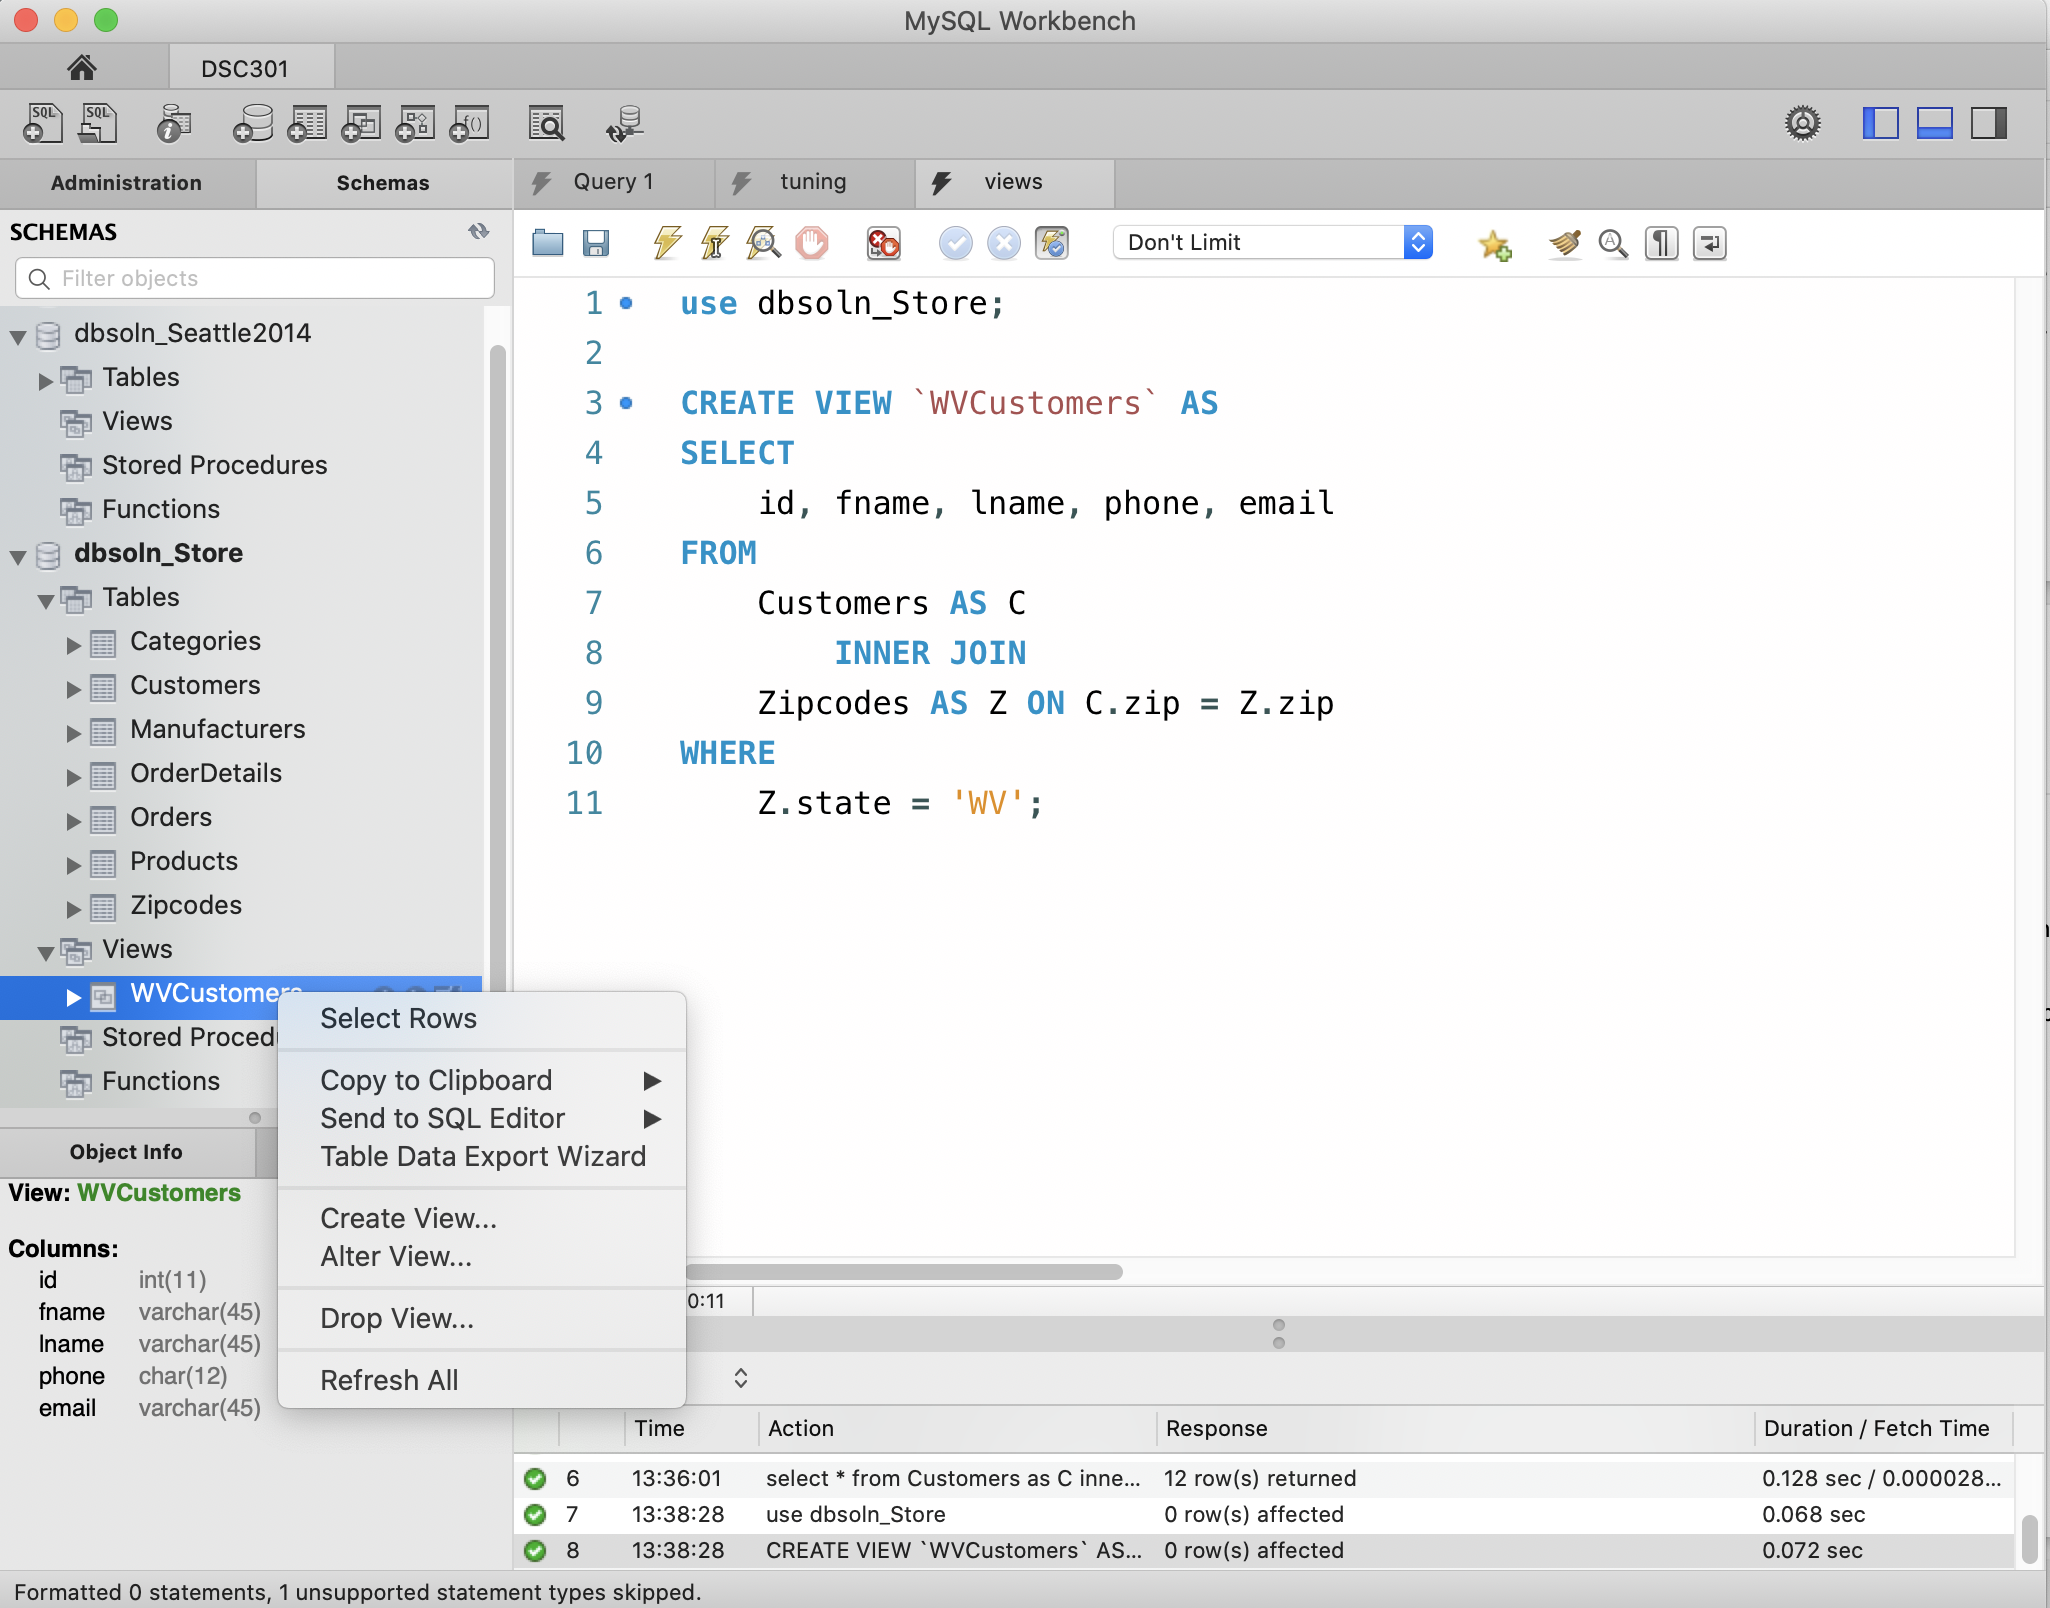
\includegraphics[scale = 0.40]{figs/mysqlwb-views} 
   \caption{MySQL Workbench Views}
   \label{fig:mysqlwb}
\end{figure}














% --------------------------------------------------
\hspace{-0.5cm}\rule[-0.101in]{\textwidth}{0.0025in}
% --------------------------------------------------
   

\subsubsection*{Updatable views - writable views}
 
 An \textit{updatable view} (as opposed to read-only views) is a view that can be used with \texttt{INSERT},  \texttt{UPDATE}, or  \texttt{DELETE} statement to update the data in a base table.
  
 Updating the underlying data from a view can be accomplished as long as: 
\begin{outline}
	\1 The view does not contain joins.
	\1 The view does not include aggregate functions.
	\1 The view does not use the \texttt{GROUP BY} or \texttt{HAVING} clause.
	\1 The view does not contain a \texttt{UNION} statement.
	\1 \texttt{DISTINCT} is not used.
\end{outline}
  
  
  
  First create a updatable view.  For example, 
  
  
\begin{lstlisting}[frame=single]  
CREATE VIEW `LowInventory` AS
    SELECT 
        id,  inventory
    FROM
        Products
    WHERE
        inventory < 5;
\end{lstlisting} 


\noindent Next, update this view by setting all inventory fields to 10.  


\begin{lstlisting}[frame=single]  
UPDATE `LowInventory` 
    SET 
        inventory = 10;
\end{lstlisting} 

  
  \noindent A clause that can prevent an update  statement from excluding rows of the view can be added when creating a view.  Specifically, the \texttt{WITH CHECK OPTION} can be added to the end of the \texttt{CREATE VIEW} statement.  
  
  
  
\begin{lstlisting}[frame=single]  
CREATE OR REPLACE VIEW <view_name> AS 
	SELECT 
		<columns> 
	FROM 
		<TableX>
	[WHERE condition]
WITH CHECK OPTION;
\end{lstlisting} 


  
    
  
  
  
  
  
  
  
  
  
  
  
  
  
  
  
%+Bibliography
%\begin{thebibliography}{99}
%\bibitem{Label1} ...
%\bibitem{Label2} ...
%\end{thebibliography}
%-Bibliography



 

\end{document}
